% Options for packages loaded elsewhere
\PassOptionsToPackage{unicode}{hyperref}
\PassOptionsToPackage{hyphens}{url}
%
\documentclass[
  man]{apa6}
\usepackage{amsmath,amssymb}
\usepackage{iftex}
\ifPDFTeX
  \usepackage[T1]{fontenc}
  \usepackage[utf8]{inputenc}
  \usepackage{textcomp} % provide euro and other symbols
\else % if luatex or xetex
  \usepackage{unicode-math} % this also loads fontspec
  \defaultfontfeatures{Scale=MatchLowercase}
  \defaultfontfeatures[\rmfamily]{Ligatures=TeX,Scale=1}
\fi
\usepackage{lmodern}
\ifPDFTeX\else
  % xetex/luatex font selection
\fi
% Use upquote if available, for straight quotes in verbatim environments
\IfFileExists{upquote.sty}{\usepackage{upquote}}{}
\IfFileExists{microtype.sty}{% use microtype if available
  \usepackage[]{microtype}
  \UseMicrotypeSet[protrusion]{basicmath} % disable protrusion for tt fonts
}{}
\makeatletter
\@ifundefined{KOMAClassName}{% if non-KOMA class
  \IfFileExists{parskip.sty}{%
    \usepackage{parskip}
  }{% else
    \setlength{\parindent}{0pt}
    \setlength{\parskip}{6pt plus 2pt minus 1pt}}
}{% if KOMA class
  \KOMAoptions{parskip=half}}
\makeatother
\usepackage{xcolor}
\usepackage{color}
\usepackage{fancyvrb}
\newcommand{\VerbBar}{|}
\newcommand{\VERB}{\Verb[commandchars=\\\{\}]}
\DefineVerbatimEnvironment{Highlighting}{Verbatim}{commandchars=\\\{\}}
% Add ',fontsize=\small' for more characters per line
\usepackage{framed}
\definecolor{shadecolor}{RGB}{248,248,248}
\newenvironment{Shaded}{\begin{snugshade}}{\end{snugshade}}
\newcommand{\AlertTok}[1]{\textcolor[rgb]{0.94,0.16,0.16}{#1}}
\newcommand{\AnnotationTok}[1]{\textcolor[rgb]{0.56,0.35,0.01}{\textbf{\textit{#1}}}}
\newcommand{\AttributeTok}[1]{\textcolor[rgb]{0.13,0.29,0.53}{#1}}
\newcommand{\BaseNTok}[1]{\textcolor[rgb]{0.00,0.00,0.81}{#1}}
\newcommand{\BuiltInTok}[1]{#1}
\newcommand{\CharTok}[1]{\textcolor[rgb]{0.31,0.60,0.02}{#1}}
\newcommand{\CommentTok}[1]{\textcolor[rgb]{0.56,0.35,0.01}{\textit{#1}}}
\newcommand{\CommentVarTok}[1]{\textcolor[rgb]{0.56,0.35,0.01}{\textbf{\textit{#1}}}}
\newcommand{\ConstantTok}[1]{\textcolor[rgb]{0.56,0.35,0.01}{#1}}
\newcommand{\ControlFlowTok}[1]{\textcolor[rgb]{0.13,0.29,0.53}{\textbf{#1}}}
\newcommand{\DataTypeTok}[1]{\textcolor[rgb]{0.13,0.29,0.53}{#1}}
\newcommand{\DecValTok}[1]{\textcolor[rgb]{0.00,0.00,0.81}{#1}}
\newcommand{\DocumentationTok}[1]{\textcolor[rgb]{0.56,0.35,0.01}{\textbf{\textit{#1}}}}
\newcommand{\ErrorTok}[1]{\textcolor[rgb]{0.64,0.00,0.00}{\textbf{#1}}}
\newcommand{\ExtensionTok}[1]{#1}
\newcommand{\FloatTok}[1]{\textcolor[rgb]{0.00,0.00,0.81}{#1}}
\newcommand{\FunctionTok}[1]{\textcolor[rgb]{0.13,0.29,0.53}{\textbf{#1}}}
\newcommand{\ImportTok}[1]{#1}
\newcommand{\InformationTok}[1]{\textcolor[rgb]{0.56,0.35,0.01}{\textbf{\textit{#1}}}}
\newcommand{\KeywordTok}[1]{\textcolor[rgb]{0.13,0.29,0.53}{\textbf{#1}}}
\newcommand{\NormalTok}[1]{#1}
\newcommand{\OperatorTok}[1]{\textcolor[rgb]{0.81,0.36,0.00}{\textbf{#1}}}
\newcommand{\OtherTok}[1]{\textcolor[rgb]{0.56,0.35,0.01}{#1}}
\newcommand{\PreprocessorTok}[1]{\textcolor[rgb]{0.56,0.35,0.01}{\textit{#1}}}
\newcommand{\RegionMarkerTok}[1]{#1}
\newcommand{\SpecialCharTok}[1]{\textcolor[rgb]{0.81,0.36,0.00}{\textbf{#1}}}
\newcommand{\SpecialStringTok}[1]{\textcolor[rgb]{0.31,0.60,0.02}{#1}}
\newcommand{\StringTok}[1]{\textcolor[rgb]{0.31,0.60,0.02}{#1}}
\newcommand{\VariableTok}[1]{\textcolor[rgb]{0.00,0.00,0.00}{#1}}
\newcommand{\VerbatimStringTok}[1]{\textcolor[rgb]{0.31,0.60,0.02}{#1}}
\newcommand{\WarningTok}[1]{\textcolor[rgb]{0.56,0.35,0.01}{\textbf{\textit{#1}}}}
\usepackage{graphicx}
\makeatletter
\def\maxwidth{\ifdim\Gin@nat@width>\linewidth\linewidth\else\Gin@nat@width\fi}
\def\maxheight{\ifdim\Gin@nat@height>\textheight\textheight\else\Gin@nat@height\fi}
\makeatother
% Scale images if necessary, so that they will not overflow the page
% margins by default, and it is still possible to overwrite the defaults
% using explicit options in \includegraphics[width, height, ...]{}
\setkeys{Gin}{width=\maxwidth,height=\maxheight,keepaspectratio}
% Set default figure placement to htbp
\makeatletter
\def\fps@figure{htbp}
\makeatother
\setlength{\emergencystretch}{3em} % prevent overfull lines
\providecommand{\tightlist}{%
  \setlength{\itemsep}{0pt}\setlength{\parskip}{0pt}}
\setcounter{secnumdepth}{-\maxdimen} % remove section numbering
% Make \paragraph and \subparagraph free-standing
\ifx\paragraph\undefined\else
  \let\oldparagraph\paragraph
  \renewcommand{\paragraph}[1]{\oldparagraph{#1}\mbox{}}
\fi
\ifx\subparagraph\undefined\else
  \let\oldsubparagraph\subparagraph
  \renewcommand{\subparagraph}[1]{\oldsubparagraph{#1}\mbox{}}
\fi
\newlength{\cslhangindent}
\setlength{\cslhangindent}{1.5em}
\newlength{\csllabelwidth}
\setlength{\csllabelwidth}{3em}
\newlength{\cslentryspacingunit} % times entry-spacing
\setlength{\cslentryspacingunit}{\parskip}
\newenvironment{CSLReferences}[2] % #1 hanging-ident, #2 entry spacing
 {% don't indent paragraphs
  \setlength{\parindent}{0pt}
  % turn on hanging indent if param 1 is 1
  \ifodd #1
  \let\oldpar\par
  \def\par{\hangindent=\cslhangindent\oldpar}
  \fi
  % set entry spacing
  \setlength{\parskip}{#2\cslentryspacingunit}
 }%
 {}
\usepackage{calc}
\newcommand{\CSLBlock}[1]{#1\hfill\break}
\newcommand{\CSLLeftMargin}[1]{\parbox[t]{\csllabelwidth}{#1}}
\newcommand{\CSLRightInline}[1]{\parbox[t]{\linewidth - \csllabelwidth}{#1}\break}
\newcommand{\CSLIndent}[1]{\hspace{\cslhangindent}#1}
\ifLuaTeX
\usepackage[bidi=basic]{babel}
\else
\usepackage[bidi=default]{babel}
\fi
\babelprovide[main,import]{english}
% get rid of language-specific shorthands (see #6817):
\let\LanguageShortHands\languageshorthands
\def\languageshorthands#1{}
% Manuscript styling
\usepackage{upgreek}
\captionsetup{font=singlespacing,justification=justified}

% Table formatting
\usepackage{longtable}
\usepackage{lscape}
% \usepackage[counterclockwise]{rotating}   % Landscape page setup for large tables
\usepackage{multirow}		% Table styling
\usepackage{tabularx}		% Control Column width
\usepackage[flushleft]{threeparttable}	% Allows for three part tables with a specified notes section
\usepackage{threeparttablex}            % Lets threeparttable work with longtable

% Create new environments so endfloat can handle them
% \newenvironment{ltable}
%   {\begin{landscape}\centering\begin{threeparttable}}
%   {\end{threeparttable}\end{landscape}}
\newenvironment{lltable}{\begin{landscape}\centering\begin{ThreePartTable}}{\end{ThreePartTable}\end{landscape}}

% Enables adjusting longtable caption width to table width
% Solution found at http://golatex.de/longtable-mit-caption-so-breit-wie-die-tabelle-t15767.html
\makeatletter
\newcommand\LastLTentrywidth{1em}
\newlength\longtablewidth
\setlength{\longtablewidth}{1in}
\newcommand{\getlongtablewidth}{\begingroup \ifcsname LT@\roman{LT@tables}\endcsname \global\longtablewidth=0pt \renewcommand{\LT@entry}[2]{\global\advance\longtablewidth by ##2\relax\gdef\LastLTentrywidth{##2}}\@nameuse{LT@\roman{LT@tables}} \fi \endgroup}

% \setlength{\parindent}{0.5in}
% \setlength{\parskip}{0pt plus 0pt minus 0pt}

% Overwrite redefinition of paragraph and subparagraph by the default LaTeX template
% See https://github.com/crsh/papaja/issues/292
\makeatletter
\renewcommand{\paragraph}{\@startsection{paragraph}{4}{\parindent}%
  {0\baselineskip \@plus 0.2ex \@minus 0.2ex}%
  {-1em}%
  {\normalfont\normalsize\bfseries\itshape\typesectitle}}

\renewcommand{\subparagraph}[1]{\@startsection{subparagraph}{5}{1em}%
  {0\baselineskip \@plus 0.2ex \@minus 0.2ex}%
  {-\z@\relax}%
  {\normalfont\normalsize\itshape\hspace{\parindent}{#1}\textit{\addperi}}{\relax}}
\makeatother

\makeatletter
\usepackage{etoolbox}
\patchcmd{\maketitle}
  {\section{\normalfont\normalsize\abstractname}}
  {\section*{\normalfont\normalsize\abstractname}}
  {}{\typeout{Failed to patch abstract.}}
\patchcmd{\maketitle}
  {\section{\protect\normalfont{\@title}}}
  {\section*{\protect\normalfont{\@title}}}
  {}{\typeout{Failed to patch title.}}
\makeatother

\usepackage{xpatch}
\makeatletter
\xapptocmd\appendix
  {\xapptocmd\section
    {\addcontentsline{toc}{section}{\appendixname\ifoneappendix\else~\theappendix\fi\\: #1}}
    {}{\InnerPatchFailed}%
  }
{}{\PatchFailed}
\keywords{Educational Outcomes, School Quality, Education}
\DeclareDelayedFloatFlavor{ThreePartTable}{table}
\DeclareDelayedFloatFlavor{lltable}{table}
\DeclareDelayedFloatFlavor*{longtable}{table}
\makeatletter
\renewcommand{\efloat@iwrite}[1]{\immediate\expandafter\protected@write\csname efloat@post#1\endcsname{}}
\makeatother
\usepackage{csquotes}
\ifLuaTeX
  \usepackage{selnolig}  % disable illegal ligatures
\fi
\IfFileExists{bookmark.sty}{\usepackage{bookmark}}{\usepackage{hyperref}}
\IfFileExists{xurl.sty}{\usepackage{xurl}}{} % add URL line breaks if available
\urlstyle{same}
\hypersetup{
  pdftitle={An Analysis of the Department of Education Quality Survey and Its Efficacy},
  pdfauthor={Andrew Bowen1, Glen Dale Davis1, Josh Forster1, Shoshana Farber1, \& Charles Ugiagbe1},
  pdflang={en-EN},
  pdfkeywords={Educational Outcomes, School Quality, Education},
  hidelinks,
  pdfcreator={LaTeX via pandoc}}

\title{An Analysis of the Department of Education Quality Survey and Its Efficacy}
\author{Andrew Bowen\textsuperscript{1}, Glen Dale Davis\textsuperscript{1}, Josh Forster\textsuperscript{1}, Shoshana Farber\textsuperscript{1}, \& Charles Ugiagbe\textsuperscript{1}}
\date{}


\shorttitle{DATA621 Final Project}

\affiliation{\vspace{0.5cm}\textsuperscript{1} City University of New York}

\abstract{%
Abstract coming soon!
}



\begin{document}
\maketitle

\hypertarget{introduction}{%
\section{Introduction}\label{introduction}}

The NYC School Survey seeks to collect data to provide an overview of New York City Schools. Beginning in 2005, the survey looks to collect demographic and achievement data for New York City Public Schools, and provide a standardized rating of various elements of school quality.

The survey has changed over the years. This change has come from recommendations of public policy analysts in order to more accurately define the quality of schools \emph{New York City Schools (2018)}. The 2020-21 academic year report provides a robust dataset defined at the school level with academic and socioeconomic data provided.

\textbf{Research Question:} This study aims to determine whether the school ratings within the NYC School Quality Survey accurately reflect educational outcomes, or if other variables related to certain schools can be used as a better proxy.

\hypertarget{literature-review}{%
\section{Literature Review}\label{literature-review}}

Measuring the input variables that impact educational outcomes is a difficult task. With so many confounding variables, it can be difficult to determine direct causal relationships that have an outsized impact

\hypertarget{data-sourcing}{%
\section{Data Sourcing}\label{data-sourcing}}

\begin{itemize}
\tightlist
\item
  \href{https://data.cityofnewyork.us/Education/2020-2021-School-Quality-Reports-High-School/26je-vkp6}{School Quality NYC 2020 - 2021}
\end{itemize}

\hypertarget{methodology}{%
\section{Methodology}\label{methodology}}

We create a 20\% holdout set of data to be used later on in order to evaluate the efficacy of our model's predictive capability. The remaining 80\% of the data is to be used for model training and exploratory data analysis (EDA).

The below plot shows the raw relationship between each survey rating (\emph{Collaborative Teaching}, \emph{Trust}, etc) and the response variables of interest: \emph{Average English/Math SAT scores} per school.

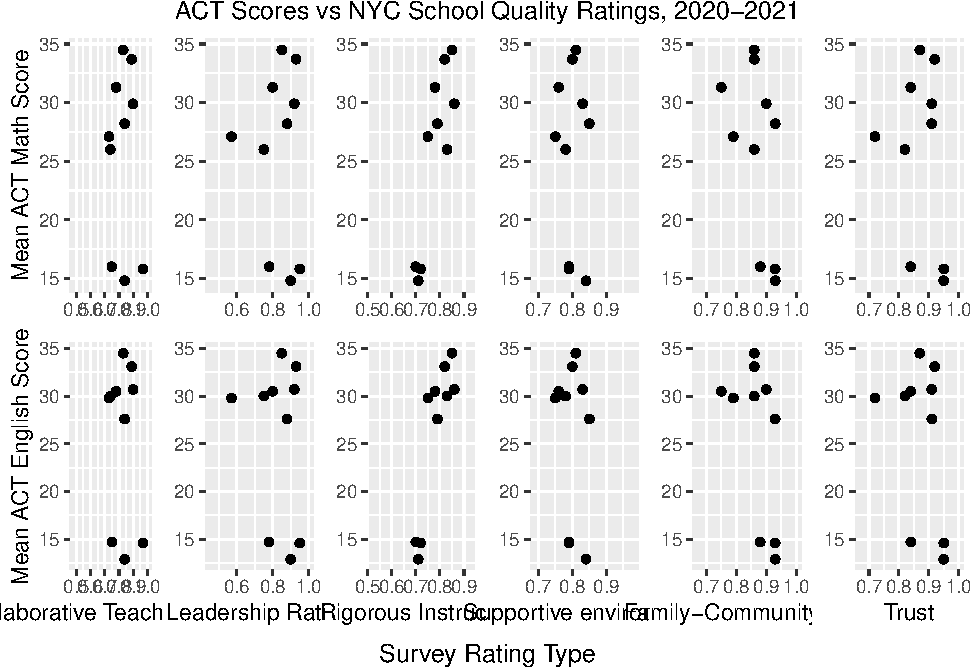
\includegraphics{final-project_files/figure-latex/plot-relationships-1.pdf}

\hypertarget{experimentation-and-results}{%
\section{Experimentation and Results}\label{experimentation-and-results}}

First, we construct a basic linear model to predict both English and Math ACT average scores for a given school.

As we see from summary stats below \(Rating \rightarrow English/Math\) models perform decently well at predicting ACT English and Math scores, respectively. We see adjusted \(R^2\) values for each academic subject below:

\begin{itemize}
\tightlist
\item
  \emph{English:} 0.76
\item
  \emph{Math:} 0.493
\end{itemize}

\begin{verbatim}
## 
## Call:
## lm(formula = english_formula, data = train)
## 
## Residuals:
##      39      90     128     132     147     193     257     259 
##  2.1072  0.1175 -0.1037 -0.7313 -0.6176  0.1158  0.7941 -1.6820 
## 
## Coefficients:
##              Estimate Std. Error t value Pr(>|t|)
## (Intercept)   -154.76      88.19  -1.755    0.330
## survey_pp_RI   118.97      32.77   3.630    0.171
## survey_pp_CT    43.29      40.36   1.073    0.478
## survey_pp_ES  -223.10     144.88  -1.540    0.367
## survey_pp_SE   -23.08     130.37  -0.177    0.888
## survey_pp_SF   -73.85      49.68  -1.486    0.377
## survey_pp_TR   370.05     271.36   1.364    0.403
## 
## Residual standard error: 2.976 on 1 degrees of freedom
##   (382 observations deleted due to missingness)
## Multiple R-squared:  0.966,  Adjusted R-squared:  0.7618 
## F-statistic:  4.73 on 6 and 1 DF,  p-value: 0.3381
\end{verbatim}

\begin{verbatim}
## 
## Call:
## lm(formula = math_formula, data = train)
## 
## Residuals:
##      39      90     128     132     147     193     257     259 
##  2.9350  0.1636 -0.1444 -1.0186 -0.8602  0.1613  1.1060 -2.3428 
## 
## Coefficients:
##              Estimate Std. Error t value Pr(>|t|)
## (Intercept)   -134.18     122.84  -1.092    0.472
## survey_pp_RI    81.91      45.65   1.794    0.324
## survey_pp_CT    46.38      56.22   0.825    0.561
## survey_pp_ES  -171.25     201.80  -0.849    0.552
## survey_pp_SE    40.36     181.58   0.222    0.861
## survey_pp_SF  -101.32      69.20  -1.464    0.381
## survey_pp_TR   296.15     377.97   0.784    0.577
## 
## Residual standard error: 4.145 on 1 degrees of freedom
##   (382 observations deleted due to missingness)
## Multiple R-squared:  0.9276, Adjusted R-squared:  0.493 
## F-statistic: 2.135 on 6 and 1 DF,  p-value: 0.4808
\end{verbatim}

We can use two variables as a proxy for the school's survey rating in predicting college persistence:

\begin{itemize}
\tightlist
\item
  Percent in Temp Housing (\texttt{temp\_housing\_pct}) - percentage of students at a given school living in NYC temporary housing
\item
  Economic Need Index (\texttt{eni\_hs\_pct\_912}) - this is a measure of the percent of students facing economic hardship at a school
\end{itemize}

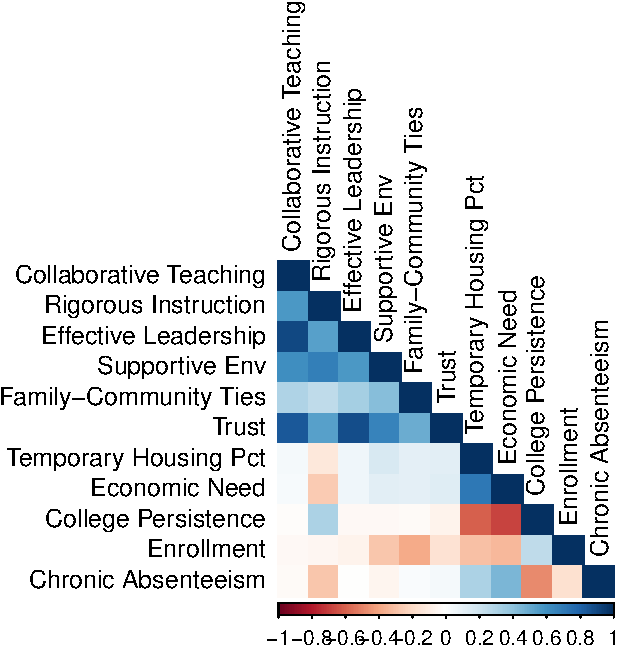
\includegraphics{final-project_files/figure-latex/unnamed-chunk-5-1.pdf}

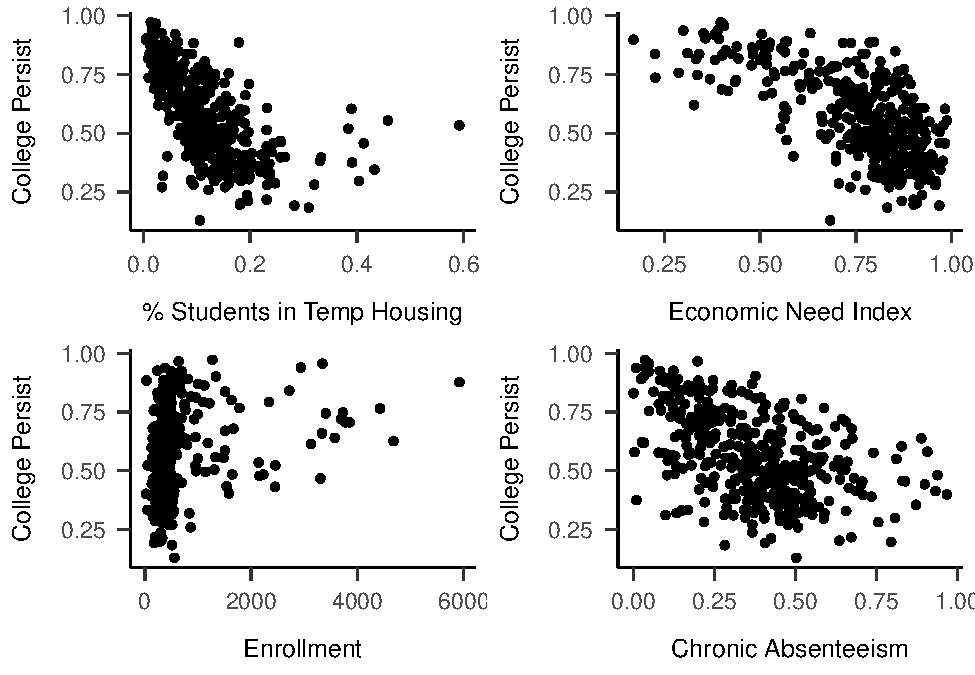
\includegraphics{final-project_files/figure-latex/unnamed-chunk-6-1.pdf}

First, we should check an assumption of linearity between our predictor and response variables.
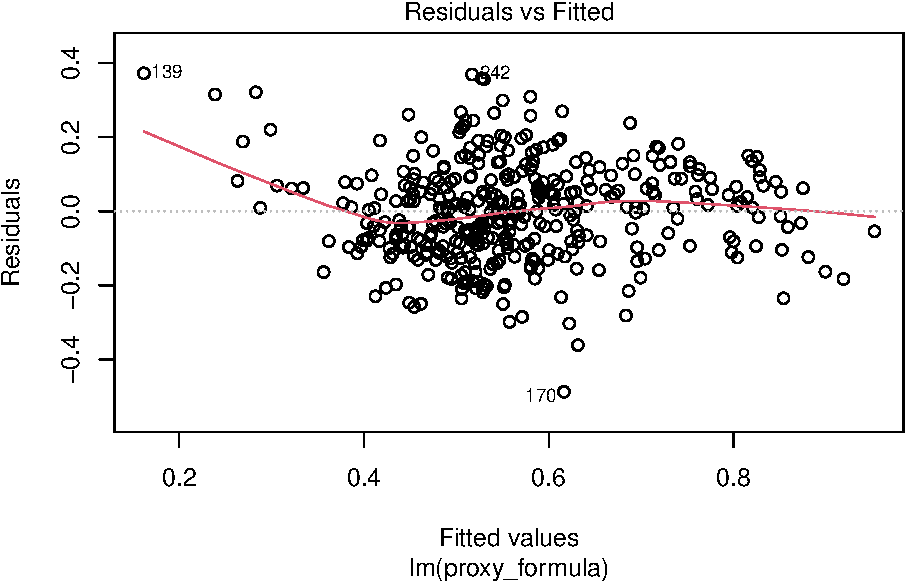
\includegraphics{final-project_files/figure-latex/unnamed-chunk-7-1.pdf}

We see a general linear relationship for schools with lower rates of students in temp housing. However, this linear relationship does \textbf{not} visually hold for schools with hisgher rates of temp housing use.

Plotting the relationship below between a school's economic need index
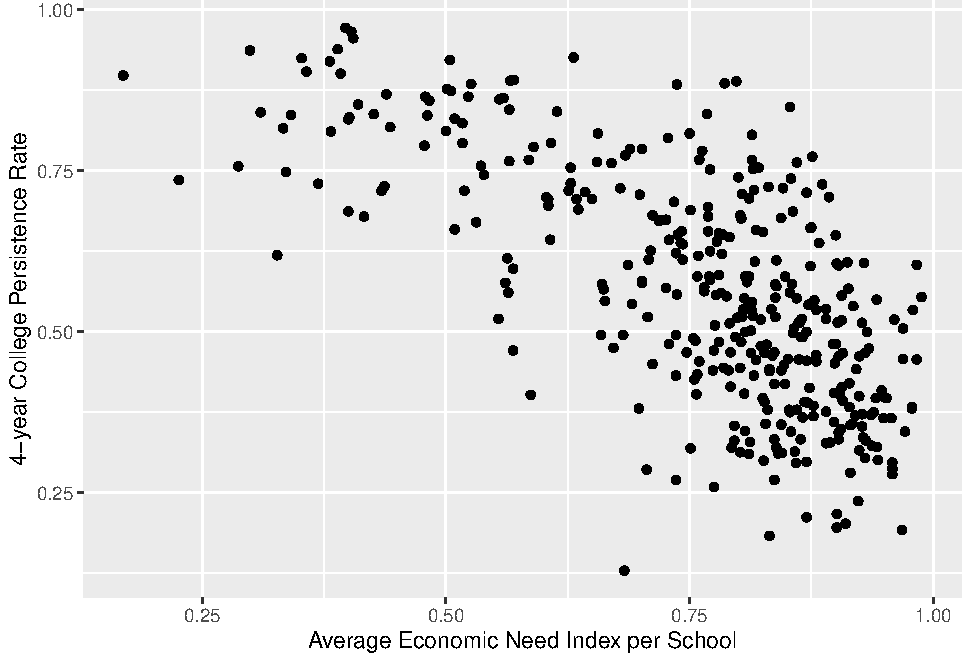
\includegraphics{final-project_files/figure-latex/unnamed-chunk-8-1.pdf}
Again, we see a non-linear relationship between our predictor (\emph{Economic Need Index}) and Outcome Variable (\emph{College Persistence Rate})

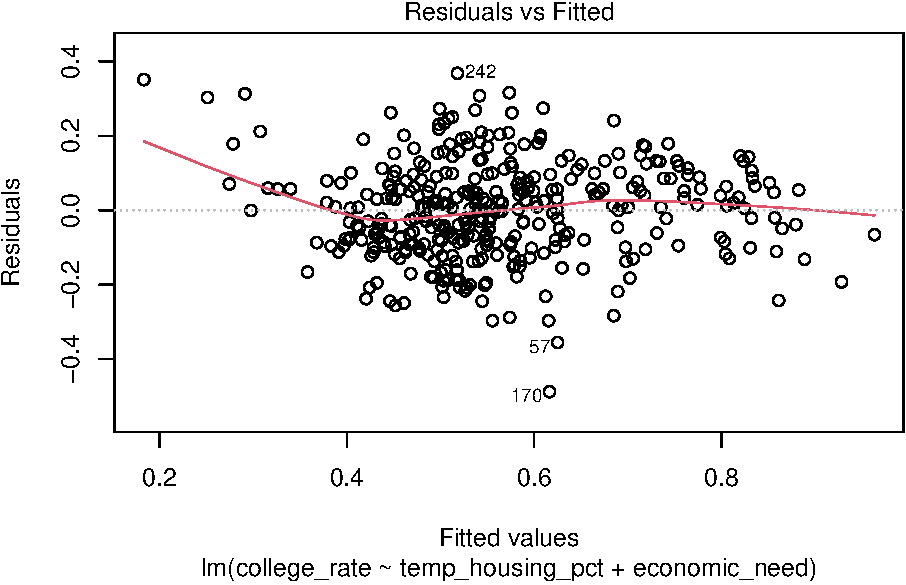
\includegraphics{final-project_files/figure-latex/unnamed-chunk-10-1.pdf} 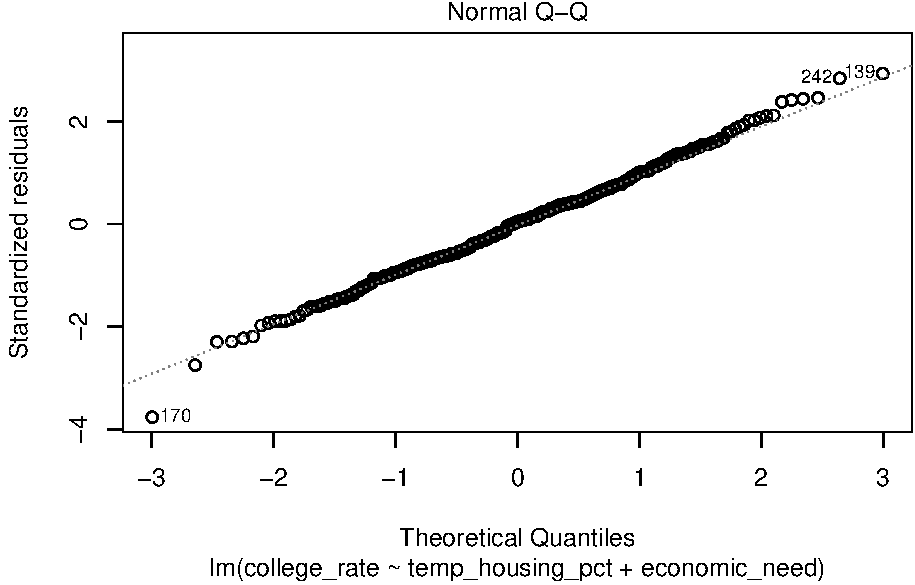
\includegraphics{final-project_files/figure-latex/unnamed-chunk-10-2.pdf} 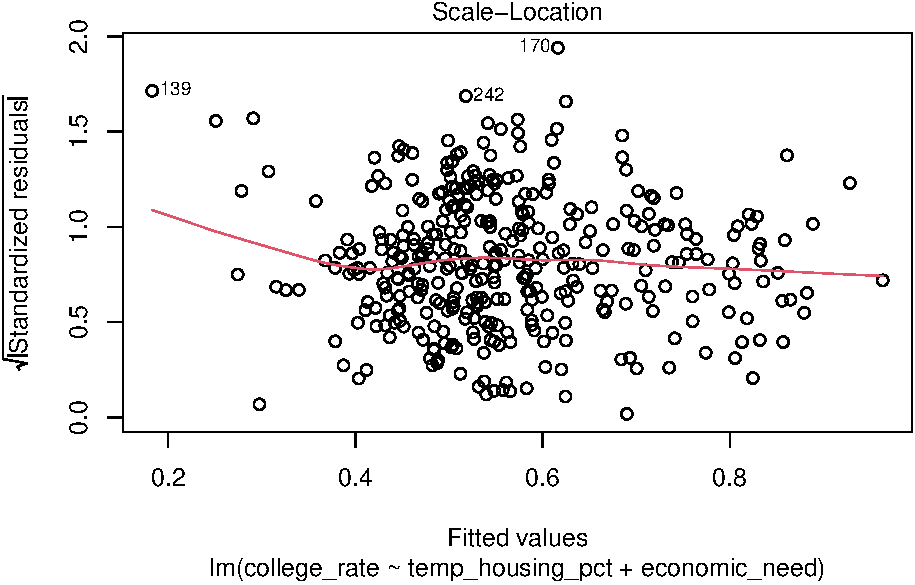
\includegraphics{final-project_files/figure-latex/unnamed-chunk-10-3.pdf} 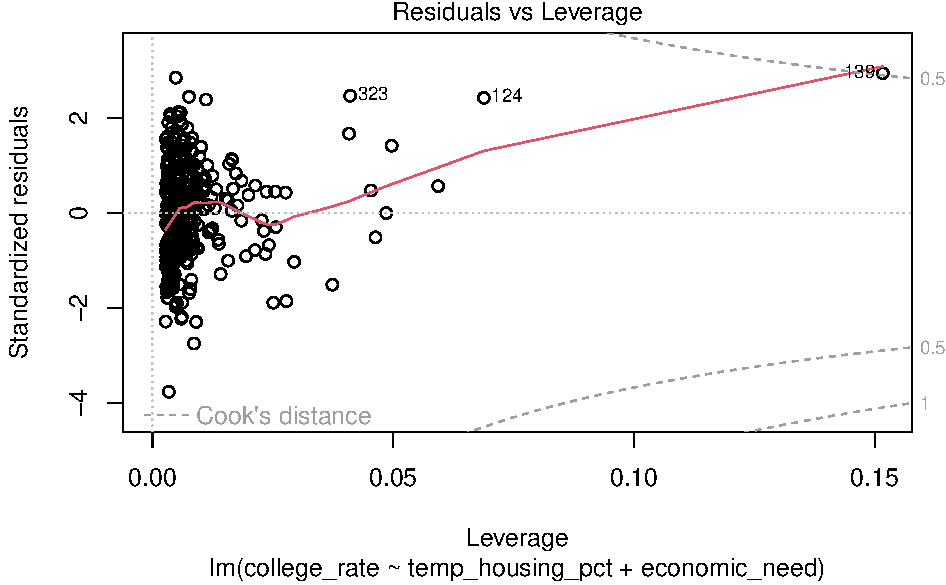
\includegraphics{final-project_files/figure-latex/unnamed-chunk-10-4.pdf}

\hypertarget{conclusion}{%
\section{Conclusion}\label{conclusion}}

\hypertarget{todo}{%
\subsection{TODO}\label{todo}}

\begin{itemize}
\tightlist
\item
  Merge/Join in ACT/SAT information by DBN
\item
  Model Selection
\end{itemize}

\newpage

\hypertarget{references}{%
\section{References}\label{references}}

\hypertarget{refs}{}
\begin{CSLReferences}{1}{0}
\leavevmode\vadjust pre{\hypertarget{ref-redesign-school-survey}{}}%
New York City Schools, T. R. A. for. (2018). \emph{{R}edesigning the {A}nnual {N}{Y}{C} {S}chool {S}urvey: {L}essons from a {R}esearch-{P}ractice {P}artnership}. \url{https://steinhardt.nyu.edu/sites/default/files/2021-01/Lessons_from_a_Research-Practice_Partnership.pdf}.

\end{CSLReferences}

\hypertarget{appendices}{%
\section{Appendices}\label{appendices}}

Below is the code used to generate this report. It's also available on \href{https://github.com/andrewbowen19/businessAnalyticsDataMiningDATA621/main}{GitHub here}

\begin{Shaded}
\begin{Highlighting}[]
\NormalTok{knitr}\SpecialCharTok{::}\NormalTok{opts\_chunk}\SpecialCharTok{$}\FunctionTok{set}\NormalTok{(}\AttributeTok{echo =} \ConstantTok{FALSE}\NormalTok{, }\AttributeTok{warning =} \ConstantTok{FALSE}\NormalTok{, }\AttributeTok{message =} \ConstantTok{FALSE}\NormalTok{)}
\FunctionTok{library}\NormalTok{(tidyverse)}
\FunctionTok{library}\NormalTok{(gridExtra)}
\FunctionTok{library}\NormalTok{(glue)}
\FunctionTok{library}\NormalTok{(}\StringTok{"papaja"}\NormalTok{)}
\FunctionTok{r\_refs}\NormalTok{(}\StringTok{"r{-}references.bib"}\NormalTok{)}
\CommentTok{\# Read in our dataset from GitHub}
\CommentTok{\# https://www.opendatanetwork.com/dataset/data.cityofnewyork.us/bm9v{-}cvch}
\NormalTok{df }\OtherTok{\textless{}{-}} \FunctionTok{read.csv}\NormalTok{(}\StringTok{"../../data/school{-}quality{-}2020{-}2021.csv"}\NormalTok{) }\CommentTok{\#"https://data.cityofnewyork.us/api/views/26je{-}vkp6/rows.csv?date=20231108")}
\NormalTok{label\_cols }\OtherTok{\textless{}{-}} \FunctionTok{c}\NormalTok{(}\StringTok{"dbn"}\NormalTok{, }\StringTok{"school\_name"}\NormalTok{, }\StringTok{"school\_type"}\NormalTok{)}
\CommentTok{\# Convert needed columns to numeric typing}
\NormalTok{df }\OtherTok{\textless{}{-}} \FunctionTok{cbind}\NormalTok{(df[, label\_cols], }\FunctionTok{as.data.frame}\NormalTok{(}\FunctionTok{lapply}\NormalTok{(df[,}\SpecialCharTok{!}\FunctionTok{names}\NormalTok{(df) }\SpecialCharTok{\%in\%}\NormalTok{ label\_cols], as.numeric)))}

\NormalTok{df}\SpecialCharTok{$}\NormalTok{college\_rate }\OtherTok{\textless{}{-}}\NormalTok{ df}\SpecialCharTok{$}\NormalTok{val\_persist3\_4yr\_all}
\NormalTok{df}\SpecialCharTok{$}\NormalTok{economic\_need }\OtherTok{\textless{}{-}}\NormalTok{ df}\SpecialCharTok{$}\NormalTok{eni\_hs\_pct\_912}
\FunctionTok{set.seed}\NormalTok{(}\DecValTok{42}\NormalTok{)}

\CommentTok{\# Adding a 20\% holdout of our input data for model evaluation later}
\NormalTok{train }\OtherTok{\textless{}{-}} \FunctionTok{subset}\NormalTok{(df[}\FunctionTok{sample}\NormalTok{(}\DecValTok{1}\SpecialCharTok{:}\FunctionTok{nrow}\NormalTok{(df)), ]) }\SpecialCharTok{\%\textgreater{}\%} \FunctionTok{sample\_frac}\NormalTok{(}\FloatTok{0.8}\NormalTok{)}


\NormalTok{test  }\OtherTok{\textless{}{-}}\NormalTok{ dplyr}\SpecialCharTok{::}\FunctionTok{anti\_join}\NormalTok{(df, train, }\AttributeTok{by =} \StringTok{\textquotesingle{}dbn\textquotesingle{}}\NormalTok{)}
\NormalTok{p1 }\OtherTok{\textless{}{-}} \FunctionTok{ggplot}\NormalTok{(df, }\FunctionTok{aes}\NormalTok{(}\AttributeTok{x=}\NormalTok{survey\_pp\_CT, }\AttributeTok{y=}\NormalTok{val\_mean\_score\_act\_math\_all)) }\SpecialCharTok{+} \FunctionTok{geom\_point}\NormalTok{() }\SpecialCharTok{+} \FunctionTok{labs}\NormalTok{(}\AttributeTok{x=}\ConstantTok{NULL}\NormalTok{, }\AttributeTok{y=}\StringTok{"Mean ACT Math Score"}\NormalTok{)}
\NormalTok{p2 }\OtherTok{\textless{}{-}} \FunctionTok{ggplot}\NormalTok{(df, }\FunctionTok{aes}\NormalTok{(}\AttributeTok{x=}\NormalTok{survey\_pp\_ES, }\AttributeTok{y=}\NormalTok{val\_mean\_score\_act\_math\_all)) }\SpecialCharTok{+} \FunctionTok{geom\_point}\NormalTok{() }\SpecialCharTok{+} \FunctionTok{labs}\NormalTok{(}\AttributeTok{x=}\ConstantTok{NULL}\NormalTok{, }\AttributeTok{y=}\ConstantTok{NULL}\NormalTok{)}
\NormalTok{p3 }\OtherTok{\textless{}{-}} \FunctionTok{ggplot}\NormalTok{(df, }\FunctionTok{aes}\NormalTok{(}\AttributeTok{x=}\NormalTok{survey\_pp\_RI, }\AttributeTok{y=}\NormalTok{val\_mean\_score\_act\_math\_all)) }\SpecialCharTok{+} \FunctionTok{geom\_point}\NormalTok{() }\SpecialCharTok{+} \FunctionTok{labs}\NormalTok{(}\AttributeTok{x=}\ConstantTok{NULL}\NormalTok{, }\AttributeTok{y=}\ConstantTok{NULL}\NormalTok{)}
\NormalTok{p4 }\OtherTok{\textless{}{-}} \FunctionTok{ggplot}\NormalTok{(df, }\FunctionTok{aes}\NormalTok{(}\AttributeTok{x=}\NormalTok{survey\_pp\_SE, }\AttributeTok{y=}\NormalTok{val\_mean\_score\_act\_math\_all)) }\SpecialCharTok{+} \FunctionTok{geom\_point}\NormalTok{() }\SpecialCharTok{+} \FunctionTok{labs}\NormalTok{(}\AttributeTok{x=}\ConstantTok{NULL}\NormalTok{, }\AttributeTok{y=}\ConstantTok{NULL}\NormalTok{)}
\NormalTok{p5 }\OtherTok{\textless{}{-}} \FunctionTok{ggplot}\NormalTok{(df, }\FunctionTok{aes}\NormalTok{(}\AttributeTok{x=}\NormalTok{survey\_pp\_SF, }\AttributeTok{y=}\NormalTok{val\_mean\_score\_act\_math\_all)) }\SpecialCharTok{+} \FunctionTok{geom\_point}\NormalTok{() }\SpecialCharTok{+} \FunctionTok{labs}\NormalTok{(}\AttributeTok{x=}\ConstantTok{NULL}\NormalTok{, }\AttributeTok{y=}\ConstantTok{NULL}\NormalTok{)}
\NormalTok{p6 }\OtherTok{\textless{}{-}} \FunctionTok{ggplot}\NormalTok{(df, }\FunctionTok{aes}\NormalTok{(}\AttributeTok{x=}\NormalTok{survey\_pp\_TR, }\AttributeTok{y=}\NormalTok{val\_mean\_score\_act\_math\_all)) }\SpecialCharTok{+} \FunctionTok{geom\_point}\NormalTok{() }\SpecialCharTok{+} \FunctionTok{labs}\NormalTok{(}\AttributeTok{x=}\ConstantTok{NULL}\NormalTok{, }\AttributeTok{y=}\ConstantTok{NULL}\NormalTok{)}

\CommentTok{\# Plot english scores}
\NormalTok{p7 }\OtherTok{\textless{}{-}} \FunctionTok{ggplot}\NormalTok{(df, }\FunctionTok{aes}\NormalTok{(}\AttributeTok{x=}\NormalTok{survey\_pp\_CT, }\AttributeTok{y=}\NormalTok{val\_mean\_score\_act\_engl\_all)) }\SpecialCharTok{+} \FunctionTok{geom\_point}\NormalTok{() }\SpecialCharTok{+} \FunctionTok{labs}\NormalTok{(}\AttributeTok{x=}\StringTok{"Collaborative Teacher Rating"}\NormalTok{,}\AttributeTok{y=}\StringTok{"Mean ACT English Score"}\NormalTok{)}
\NormalTok{p8 }\OtherTok{\textless{}{-}} \FunctionTok{ggplot}\NormalTok{(df, }\FunctionTok{aes}\NormalTok{(}\AttributeTok{x=}\NormalTok{survey\_pp\_ES, }\AttributeTok{y=}\NormalTok{val\_mean\_score\_act\_engl\_all)) }\SpecialCharTok{+} \FunctionTok{geom\_point}\NormalTok{() }\SpecialCharTok{+} \FunctionTok{labs}\NormalTok{(}\AttributeTok{x=}\StringTok{"Leadership Rating"}\NormalTok{, }\AttributeTok{y=}\ConstantTok{NULL}\NormalTok{)}
\NormalTok{p9 }\OtherTok{\textless{}{-}} \FunctionTok{ggplot}\NormalTok{(df, }\FunctionTok{aes}\NormalTok{(}\AttributeTok{x=}\NormalTok{survey\_pp\_RI, }\AttributeTok{y=}\NormalTok{val\_mean\_score\_act\_engl\_all)) }\SpecialCharTok{+} \FunctionTok{geom\_point}\NormalTok{() }\SpecialCharTok{+} \FunctionTok{labs}\NormalTok{(}\AttributeTok{x=}\StringTok{"Rigorous Instruction"}\NormalTok{, }\AttributeTok{y=}\ConstantTok{NULL}\NormalTok{)}
\NormalTok{p10 }\OtherTok{\textless{}{-}} \FunctionTok{ggplot}\NormalTok{(df, }\FunctionTok{aes}\NormalTok{(}\AttributeTok{x=}\NormalTok{survey\_pp\_SE, }\AttributeTok{y=}\NormalTok{val\_mean\_score\_act\_engl\_all)) }\SpecialCharTok{+} \FunctionTok{geom\_point}\NormalTok{() }\SpecialCharTok{+} \FunctionTok{labs}\NormalTok{(}\AttributeTok{x=}\StringTok{"Supportive environment"}\NormalTok{, }\AttributeTok{y=}\ConstantTok{NULL}\NormalTok{)}
\NormalTok{p11 }\OtherTok{\textless{}{-}} \FunctionTok{ggplot}\NormalTok{(df, }\FunctionTok{aes}\NormalTok{(}\AttributeTok{x=}\NormalTok{survey\_pp\_SF, }\AttributeTok{y=}\NormalTok{val\_mean\_score\_act\_engl\_all)) }\SpecialCharTok{+} \FunctionTok{geom\_point}\NormalTok{() }\SpecialCharTok{+} \FunctionTok{labs}\NormalTok{(}\AttributeTok{x=}\StringTok{"Family{-}Community Ties"}\NormalTok{, }\AttributeTok{y=}\ConstantTok{NULL}\NormalTok{)}
\NormalTok{p12 }\OtherTok{\textless{}{-}} \FunctionTok{ggplot}\NormalTok{(df, }\FunctionTok{aes}\NormalTok{(}\AttributeTok{x=}\NormalTok{survey\_pp\_TR, }\AttributeTok{y=}\NormalTok{val\_mean\_score\_act\_engl\_all)) }\SpecialCharTok{+} \FunctionTok{geom\_point}\NormalTok{() }\SpecialCharTok{+} \FunctionTok{labs}\NormalTok{(}\AttributeTok{x=}\StringTok{"Trust"}\NormalTok{, }\AttributeTok{y=}\ConstantTok{NULL}\NormalTok{)}

\CommentTok{\# Panel plot}
\FunctionTok{grid.arrange}\NormalTok{(}
\NormalTok{  p1, p2,}
\NormalTok{  p3, p4,}
\NormalTok{  p5, p6,}
\NormalTok{  p7, p8,}
\NormalTok{  p9, p10,}
\NormalTok{  p11, p12,}
  \AttributeTok{nrow=}\DecValTok{2}\NormalTok{,}
  \AttributeTok{ncol=}\DecValTok{6}\NormalTok{,}
  \AttributeTok{top =} \StringTok{"ACT Scores vs NYC School Quality Ratings, 2020{-}2021"}\NormalTok{,}
  \AttributeTok{bottom=}\StringTok{"Survey Rating Type"}
\NormalTok{)}

\NormalTok{english\_formula }\OtherTok{\textless{}{-}}\NormalTok{ val\_mean\_score\_act\_engl\_all }\SpecialCharTok{\textasciitilde{}}\NormalTok{ survey\_pp\_RI }\SpecialCharTok{+}\NormalTok{ survey\_pp\_CT }\SpecialCharTok{+}\NormalTok{ survey\_pp\_ES }\SpecialCharTok{+}\NormalTok{ survey\_pp\_SE }\SpecialCharTok{+}\NormalTok{ survey\_pp\_SF }\SpecialCharTok{+}\NormalTok{ survey\_pp\_TR}

\NormalTok{math\_formula }\OtherTok{\textless{}{-}}\NormalTok{  val\_mean\_score\_act\_math\_all }\SpecialCharTok{\textasciitilde{}}\NormalTok{ survey\_pp\_RI }\SpecialCharTok{+}\NormalTok{ survey\_pp\_CT }\SpecialCharTok{+}\NormalTok{ survey\_pp\_ES }\SpecialCharTok{+}\NormalTok{ survey\_pp\_SE }\SpecialCharTok{+}\NormalTok{ survey\_pp\_SF }\SpecialCharTok{+}\NormalTok{ survey\_pp\_TR}

\CommentTok{\# Create lineaer model to predict english and math scores based on sruvey ratings}
\NormalTok{lm\_english }\OtherTok{\textless{}{-}} \FunctionTok{lm}\NormalTok{(english\_formula, }\AttributeTok{data=}\NormalTok{train)}
\NormalTok{lm\_math }\OtherTok{\textless{}{-}} \FunctionTok{lm}\NormalTok{(math\_formula, }\AttributeTok{data=}\NormalTok{train)}
\FunctionTok{summary}\NormalTok{(lm\_english)}
\FunctionTok{summary}\NormalTok{(lm\_math)}
\FunctionTok{hist}\NormalTok{(train}\SpecialCharTok{$}\NormalTok{college\_rate)}
\FunctionTok{ggplot}\NormalTok{(train, }\FunctionTok{aes}\NormalTok{(}\AttributeTok{x=}\NormalTok{temp\_housing\_pct)) }\SpecialCharTok{+} \FunctionTok{geom\_histogram}\NormalTok{() }\SpecialCharTok{+} \FunctionTok{labs}\NormalTok{(}\AttributeTok{x=}\StringTok{"\% of Students in Temporary Housing"}\NormalTok{, }\AttributeTok{y=}\StringTok{"Number of NYC Schools"}\NormalTok{)}

\FunctionTok{ggplot}\NormalTok{(train, }\FunctionTok{aes}\NormalTok{(}\AttributeTok{x=}\NormalTok{temp\_housing\_pct, }\AttributeTok{y=}\NormalTok{college\_rate)) }\SpecialCharTok{+} \FunctionTok{geom\_point}\NormalTok{() }\SpecialCharTok{+} \FunctionTok{labs}\NormalTok{(}\AttributeTok{x=}\StringTok{"\% of Students in Temporary Housing"}\NormalTok{, }\AttributeTok{y=}\StringTok{"4{-}year College Persistence Rate"}\NormalTok{)}

\FunctionTok{ggplot}\NormalTok{(train, }\FunctionTok{aes}\NormalTok{(}\AttributeTok{x=}\NormalTok{economic\_need, }\AttributeTok{y=}\NormalTok{college\_rate)) }\SpecialCharTok{+} \FunctionTok{geom\_point}\NormalTok{() }\SpecialCharTok{+}
  \FunctionTok{labs}\NormalTok{(}\AttributeTok{x=}\StringTok{"Average Economic Need Index per School"}\NormalTok{, }\AttributeTok{y=}\StringTok{"4{-}year College Persistence Rate"}\NormalTok{)}
\NormalTok{proxy\_lm }\OtherTok{\textless{}{-}} \FunctionTok{lm}\NormalTok{(college\_rate }\SpecialCharTok{\textasciitilde{}}\NormalTok{ temp\_housing\_pct }\SpecialCharTok{+}\NormalTok{ economic\_need, train)}
\FunctionTok{plot}\NormalTok{(proxy\_lm)}
\end{Highlighting}
\end{Shaded}


\end{document}
